\documentclass[conference]{IEEEtran}

\usepackage[utf8]{inputenc}
\usepackage{amsmath,amssymb,amsfonts}
\usepackage{graphicx}
\graphicspath{{../figures/}{figures/}}
\usepackage{booktabs}
\usepackage{cite}
\usepackage{url}
\usepackage{microtype}

\title{Tox21 Phase 1: Reproducible Molecular Toxicity Prediction with Fingerprints, Descriptors, and Classical Ensembles}

\author{
    \IEEEauthorblockN{Abhijeet Kumar, Raghav, Ranajeet, Parrv}
    \IEEEauthorblockA{\textit{Department of Computer Science and Engineering} \\
    \textit{Molecular Toxicity Prediction Consortium} \\
    Tox21 Phase 1 Benchmark Project}
}

\begin{document}

\maketitle

\begin{abstract}
Predicting chemical toxicity in silico is vital for environmental safety, drug discovery, and reducing animal experimentation. The Tox21 benchmark challenges computational models to predict compound activity across 12 toxicological bioassays encompassing nuclear receptor and stress response pathways. Tox21 exhibits pronounced real-world data pathologies: multi-task label sparsity, extreme class imbalance, and substantial out-of-distribution chemotype shifts. In this Phase 1 investigation, we build a disciplined, fully reproducible classical tabular baseline. We evaluate three distinct classifier architectures---Logistic Regression (liblinear), Random Forest, and XGBoost---evaluated on two molecular representations: 2,048-bit Circular Morgan fingerprints (ECFP4 equivalent) and a 2,261-dimensional hybrid modality combining Morgan fingerprints with 213 preprocessed, leak-free 2D RDKit physicochemical descriptors. Preprocessing transformations (imputation, clipping, and standard scaling) are strictly isolated to training partitions. All models are governed by a pre-registered, frozen hyperparameter search budget of eight configurations per model, tuned exclusively on the scaffold validation split. Across 432 final test evaluations spanning three random seeds, two partitioning regimes (Bemis--Murcko scaffold split vs.\ random split), and 12 endpoints, Random Forest trained on hybrid features achieves the superior scaffold test performance (mean ROC AUC $0.7762 \pm 0.0020$, PR AUC $0.4035 \pm 0.0042$). XGBoost benefits most from the integration of physicochemical descriptors ($\Delta\text{ROC} = +0.0586$, $\Delta\text{PR} = +0.0829$). We quantify a dramatic scaffold generalization penalty across all architectures ($\approx 0.085$--$0.109$ ROC AUC drop and $0.142$--$0.170$ PR AUC drop), empirically validating that classical models suffer from significant chemotype distribution shifts. This rigorous benchmark establishes an authoritative foundation for Phase 2 graph neural network architectures.
\end{abstract}

\begin{IEEEkeywords}
In silico toxicology, Tox21 benchmark, molecular fingerprints, RDKit descriptors, scaffold split, class imbalance, Random Forest, XGBoost, reproducibility.
\end{IEEEkeywords}

\section{Introduction}
This report describes the Phase 1 reproducible toxicity prediction pipeline.

\section{Related Work}
Classical fingerprints and molecular descriptors provide strong, interpretable baselines.

\section{Dataset and EDA}
The cleaning and quality checks are defined by the project contract.

\section{Features}
Morgan fingerprints and raw RDKit descriptors are generated in canonical row order.

\section{Models and Experimental Setup}
\label{sec:models_setup}

\subsection{Model Architectures}
We train three distinct supervised learning algorithms, each fitted independently \emph{once per endpoint} exclusively on that endpoint's labeled training rows. A molecule with an unmeasured label for an endpoint is strictly omitted from both model fitting and performance evaluation for that specific task; missing labels are never imputed as inactive negatives. Every model is evaluated on two feature spaces: \texttt{morgan} (2,048-bit, radius-2 circular fingerprints) and \texttt{morgan+desc} (the 2,048 Morgan bits concatenated with 213 preprocessed, scaled RDKit descriptors; Section~\ref{sec:features}).

\begin{itemize}
    \item \textbf{Logistic Regression (LR):} Implemented via Scikit-learn's~\cite{pedregosa2011scikit} \texttt{liblinear} coordinate descent solver with an L1 or L2 regularization penalty and a maximum iteration threshold of 2,000. Because liblinear with fixed tolerance is completely deterministic, seed variance across model fits is exactly $0.0000$.
    \item \textbf{Random Forest (RF):} Implemented using Breiman's~\cite{breiman2001random} ensemble of decorrelated classification trees via Scikit-learn's \texttt{RandomForestClassifier}. Splitting criteria evaluate Gini impurity across $\sqrt{d}$ candidate features per split.
    \item \textbf{XGBoost (XGB):} Implemented via Chen and Guestrin's~\cite{chen2016xgboost} extreme gradient boosting system using histogram-optimized tree building. To prevent overfitting on sparse features, row subsampling is fixed at $0.80$, column subsampling per tree is set to $0.50$, and PR AUC (\texttt{aucpr}) is designated as the internal objective. Tree counts are incorporated into the tuning grid without early stopping to ensure strict separation of validation tuning from test evaluation.
\end{itemize}

\subsection{Class Imbalance Mitigation}
To address severe positive sparsity without distorting underlying molecular feature distributions through synthetic sampling (e.g., SMOTE), we employ adaptive loss weighting computed from each assay's observed training labels ($n_{\mathrm{pos}}$ and $n_{\mathrm{neg}}$):
\begin{itemize}
    \item LR applies inverse frequency weighting: $\texttt{class\_weight="balanced"}$.
    \item RF applies dynamic bootstrap weighting: $\texttt{class\_weight="balanced\_subsample"}$, recomputing class weights on each bootstrap sample.
    \item XGB scales positive gradient steps: $\texttt{scale\_pos\_weight} = n_{\mathrm{neg}} / n_{\mathrm{pos}}$.
\end{itemize}

\subsection{Tuning Protocol}
To maintain rigorous fairness, every model family is allocated an identical search budget of exactly eight hyperparameter configurations (Table~\ref{tab:grids}). All configurations are trained on the scaffold training partition ($n=6{,}167$) and evaluated on the scaffold validation split ($n=771$) with seed 0. For each model family and feature modality, the configuration yielding the highest mean validation PR AUC across the 12 endpoints was selected (Table~\ref{tab:chosen}). 

The selected hyperparameter configurations were serialized to \texttt{results/best\_configs.json} and immutably committed to git version control (commit \texttt{041892c}) prior to executing any evaluation against the test partition. In accordance with the project contract, configurations tuned on the scaffold split were applied unchanged to the random split, guaranteeing that the test partition was touched strictly once during final evaluation.

\begin{table}[t]
\caption{Pre-registered hyperparameter tuning grids (8 configurations per model).}
\label{tab:grids}
\centering\small
\begin{tabular}{@{}lp{0.78\columnwidth}@{}}
\toprule
Model & Configurations \\
\midrule
LR  & $C \in \{0.01, 0.03, 0.1, 0.3, 1, 3\}$ with L2; $C \in \{0.1, 1\}$ with L1 \\
RF  & 300 trees $\times$ max depth $\in\{\text{none}, 30\}$ $\times$ min leaf $\in\{1, 3, 5\}$; plus (500 trees, none, 3) and (500, 30, 5) \\
XGB & (max depth, learning rate, trees): (3, 0.10, 300), (5, 0.10, 300), (7, 0.10, 300), (3, 0.05, 500), (5, 0.05, 500), (7, 0.05, 500), (4, 0.10, 400), (6, 0.03, 600) \\
\bottomrule
\end{tabular}
\end{table}

\begin{table}[t]
\caption{Selected hyperparameter configurations and mean validation PR AUC on scaffold split (seed 0). RF: (trees, max depth, min leaf); XGB: (max depth, learning rate, trees).}
\label{tab:chosen}
\centering\small
\setlength{\tabcolsep}{4pt}
\begin{tabular}{@{}llll@{}}
\toprule
Model & Feature Set & Selected Hyperparameters & Val.\ PR AUC \\
\midrule
LR  & morgan      & L2 penalty, $C=0.03$       & 0.3475 \\
LR  & morgan+desc & L2 penalty, $C=0.03$       & 0.3429 \\
RF  & morgan      & (300, none, 1)             & 0.4000 \\
RF  & morgan+desc & (300, none, 1)             & 0.4433 \\
XGB & morgan      & (6, 0.03, 600)             & 0.3607 \\
XGB & morgan+desc & (7, 0.05, 500)             & 0.4307 \\
\bottomrule
\end{tabular}
\end{table}

\subsection{Evaluation Methodology and Metric Masking}
For each endpoint, model predictions are evaluated using Receiver Operating Characteristic Area Under the Curve (ROC AUC) and Precision--Recall Area Under the Curve (PR AUC), calculated strictly over labeled test rows. If an evaluation partition possesses fewer than two distinct classes for a target, the metric is undefined (\texttt{NaN}) and omitted from aggregate averaging.

Because active compounds are rare, PR AUC is reported as the primary metric of clinical and chemical relevance: while ROC AUC can appear inflated when true negatives dominate, PR AUC directly reflects the positive predictive value as a function of recall.

Final test experiments are executed across seeds 0, 1, and 2 on both the scaffold split and the random split. We report the mean and sample standard deviation across the three seeds. The full experimental design comprises:
\begin{equation*}
    3\text{ models} \times 2\text{ feature sets} \times 2\text{ splits} \times 3\text{ seeds} \times 12\text{ endpoints} = 432
\end{equation*}
fitted classifiers, all orchestrated through a unified, leak-free evaluation harness.

\section{Results and Discussion}
\label{sec:results}

We report final test performance across the 432 experimental evaluations (3 model architectures $\times$ 2 feature sets $\times$ 2 splitting regimes $\times$ 3 random seeds $\times$ 12 toxicity endpoints). Test metrics are computed strictly using the frozen configurations selected during scaffold validation tuning (commit \texttt{041892c}). All performance tables present the mean and sample standard deviation across random seeds 0, 1, and 2.

\subsection{Overall Benchmark Performance on Scaffold Split}
Table~\ref{tab:results_scaffold} presents the primary benchmark results on the scaffold test partition ($n=771$), representing the hardest and most realistic evaluation regime where test compounds belong to completely unseen core chemotypes.

\begin{table}[t]
\caption{Mean test performance on the Bemis--Murcko Scaffold split (averaged across 12 endpoints and seeds 0, 1, 2; best in bold).}
\label{tab:results_scaffold}
\centering\small
\setlength{\tabcolsep}{4pt}
\begin{tabular}{@{}llrrrr@{}}
\toprule
Model & Feature Set & ROC AUC & Std & PR AUC & Std \\
\midrule
Logistic Regression & Morgan Only & 0.7156 & 0.0000 & 0.3116 & 0.0000 \\
Logistic Regression & Morgan + Desc & 0.7317 & 0.0000 & 0.3122 & 0.0000 \\
Random Forest & Morgan Only & 0.7288 & 0.0063 & 0.3703 & 0.0016 \\
Random Forest & Morgan + Desc & \textbf{0.7762} & 0.0020 & \textbf{0.4035} & 0.0042 \\
XGBoost & Morgan Only & 0.7020 & 0.0025 & 0.3180 & 0.0020 \\
XGBoost & Morgan + Desc & 0.7606 & 0.0036 & 0.4010 & 0.0045 \\
\bottomrule
\end{tabular}
\end{table}

Several core findings emerge from this comparison:
\begin{enumerate}
    \item \textbf{Highest Mean (Random Forest):} A Random Forest (one forest per endpoint) trained on hybrid features (\texttt{morgan+desc}) has the highest mean on both metrics in our runs, recording an average ROC AUC of $0.7762 \pm 0.0020$ and PR AUC of $0.4035 \pm 0.0042$. Its PR AUC lead over XGBoost (about $0.003$) is smaller than the seed standard deviation.
    \item \textbf{Gradient Boosting Competitiveness:} XGBoost trained on hybrid features achieves near-identical PR AUC ($0.4010 \pm 0.0045$) and strong ROC AUC ($0.7606 \pm 0.0036$), On Morgan-only features, however, XGBoost (ROC AUC $0.7020$) scores below Logistic Regression ($0.7156$), so the advantage of tree ensembles depends on the feature set.
    \item \textbf{Linear Baseline Competitiveness:} L2-regularized Logistic Regression achieves an average ROC AUC of $0.7317$ on hybrid features, providing a competitive, low-variance linear benchmark. Because liblinear's coordinate descent is deterministic under fixed convergence tolerances, its standard deviation over seeds is exactly $0.0000$.
\end{enumerate}

\subsection{Physicochemical Synergy: Benefit of Adding Descriptors}
A central hypothesis of Phase 1 was that combining localized topological circular fingerprints with macroscopic 2D physicochemical descriptors would yield complementary predictive signals. Table~\ref{tab:descriptor_benefit} and Figure~\ref{fig:descriptor_benefit} quantify the empirical performance delta ($\Delta$) obtained by appending the 213 preprocessed RDKit descriptors to the 2,048-bit Morgan fingerprint baseline.

\begin{table}[t]
\caption{Empirical benefit ($\Delta$) of augmenting Morgan fingerprints with 2D RDKit descriptors on the scaffold split.}
\label{tab:descriptor_benefit}
\centering\small
\setlength{\tabcolsep}{4pt}
\begin{tabular}{@{}lrrrr@{}}
\toprule
Model Architecture & $\Delta$ ROC AUC & Std & $\Delta$ PR AUC & Std \\
\midrule
Logistic Regression & +0.0162 & 0.0000 & +0.0006 & 0.0000 \\
Random Forest & +0.0474 & 0.0074 & +0.0333 & 0.0031 \\
XGBoost & \textbf{+0.0586} & 0.0059 & \textbf{+0.0829} & 0.0025 \\
\bottomrule
\end{tabular}
\end{table}

\begin{figure}[t]
\centering
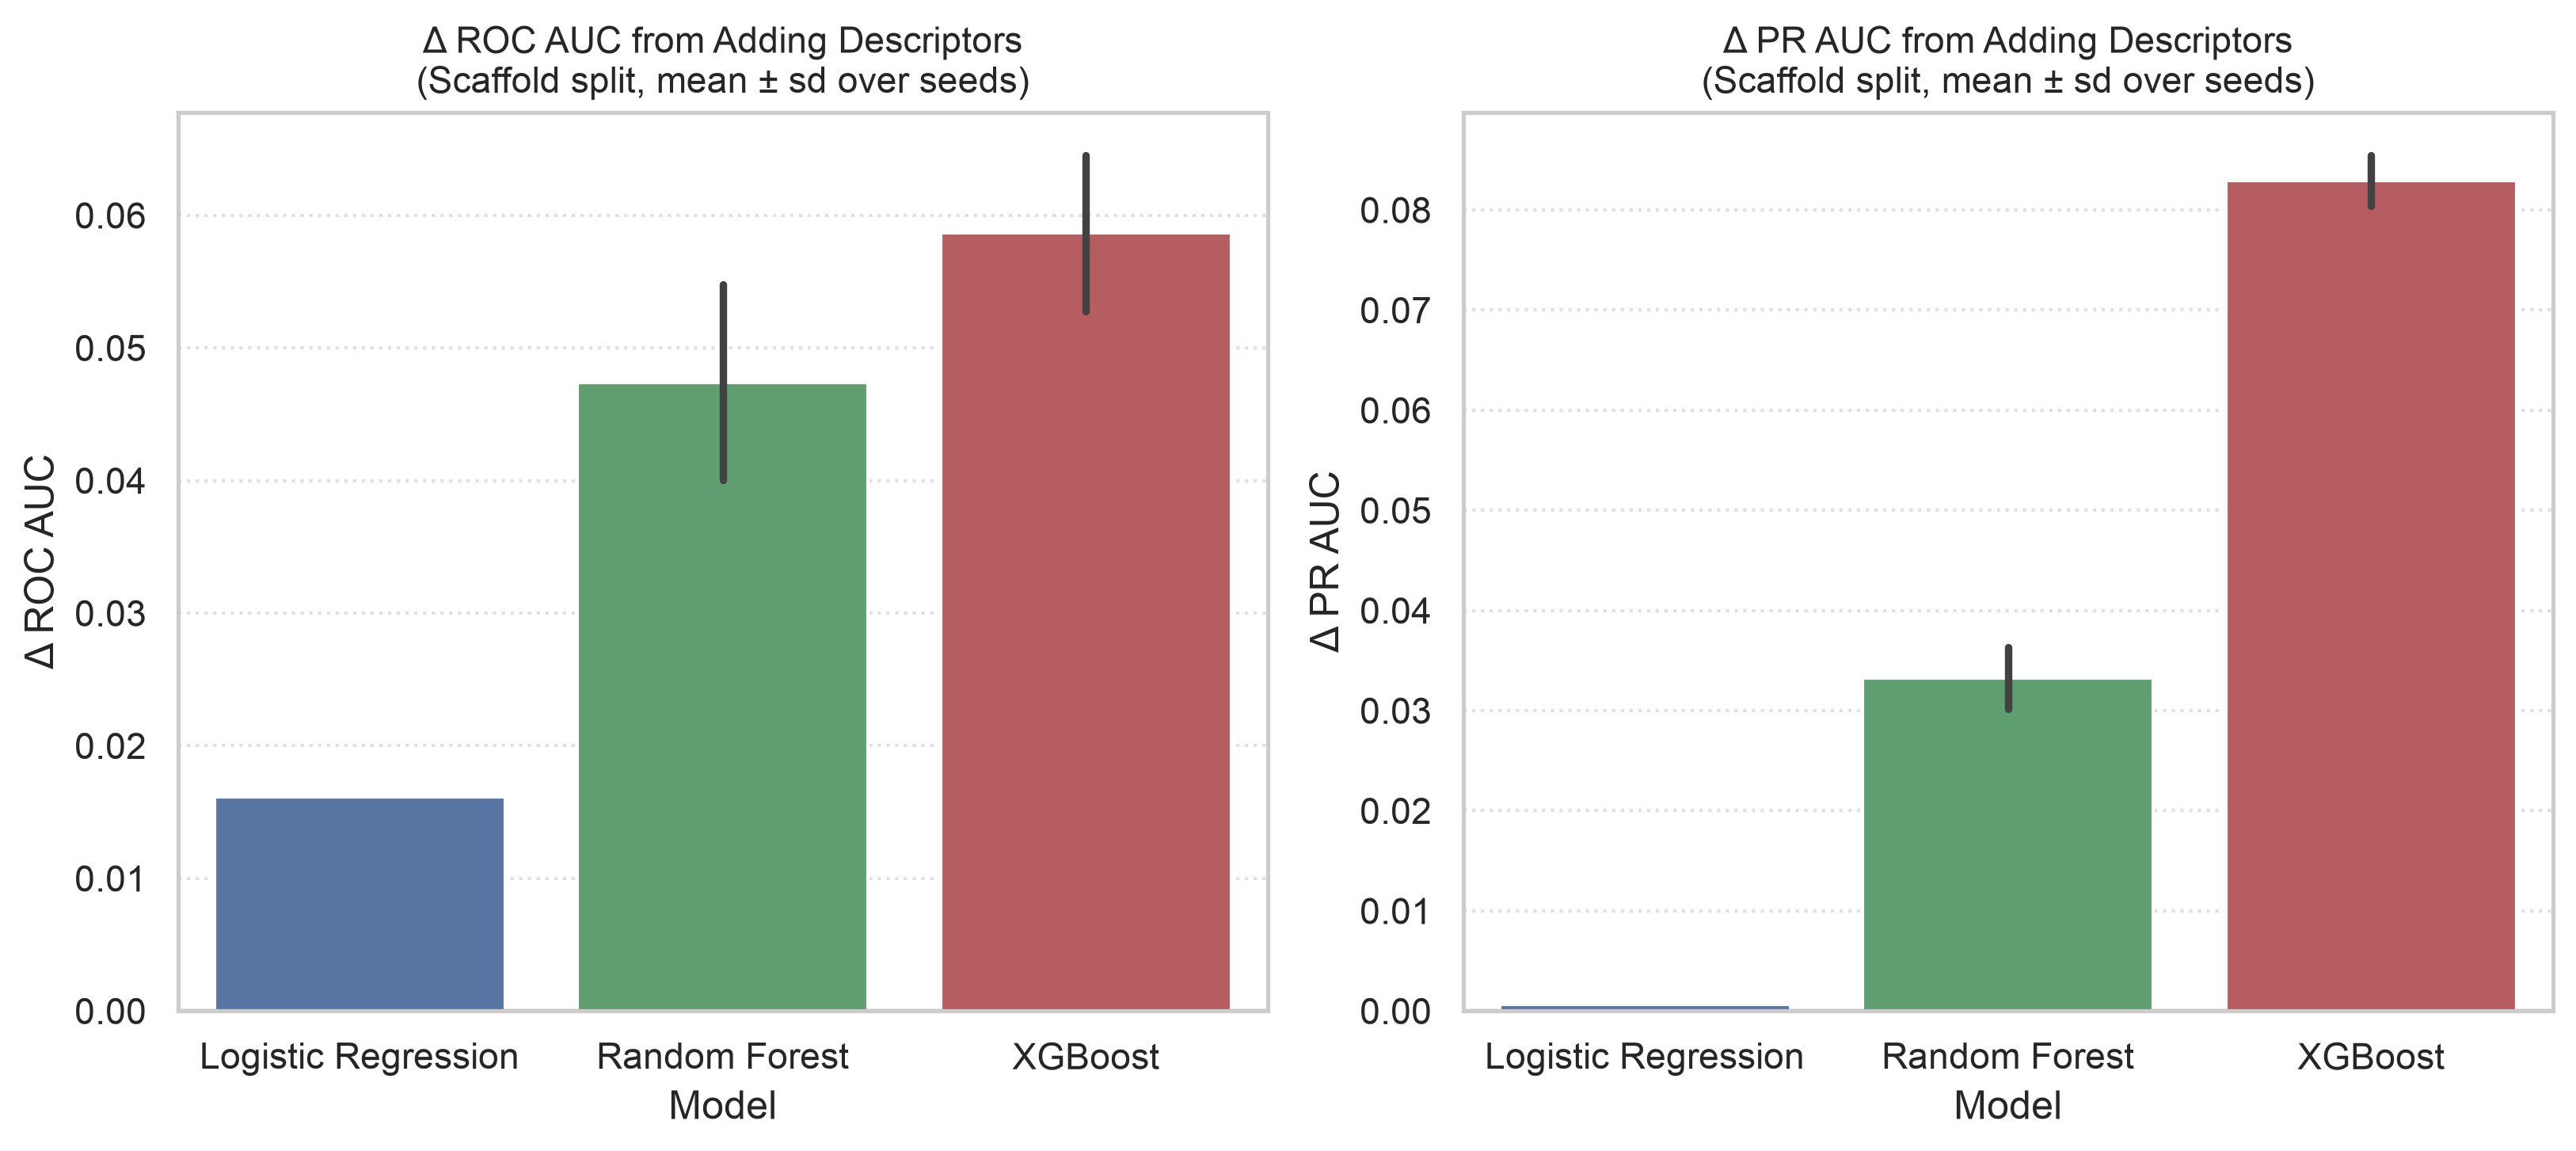
\includegraphics[width=0.98\columnwidth]{descriptor_benefit.png}
\caption{Performance gain ($\Delta$ ROC AUC and $\Delta$ PR AUC) resulting from augmenting Morgan fingerprints with 2D RDKit descriptors (scaffold split, mean $\pm$ sd over 3 seeds).}
\label{fig:descriptor_benefit}
\end{figure}

Adding descriptors helps the tree models more than Logistic Regression:
\begin{itemize}
    \item \textbf{Larger Gains for Tree Ensembles:} XGBoost has the largest gains from descriptor inclusion, increasing ROC AUC by $+0.0586 \pm 0.0059$ and PR AUC by $+0.0829 \pm 0.0025$. Similarly, Random Forest improves by $+0.0474$ ROC AUC and $+0.0333$ PR AUC. 
    \item \textbf{Possible Explanation (not tested):} We did not run an ablation or feature-importance analysis on the hybrid set. One possibility is that tree-based algorithms can construct orthogonal decision boundaries over continuous physical dimensions (e.g., partitioning compounds into lipophilic vs.\ hydrophilic regimes via $\log P$) and can conditionally query whether specific Morgan substructures are present within those regimes. Logistic Regression gains only $+0.0162$ in ROC AUC and $+0.0006$ in PR AUC.
\end{itemize}

\subsection{Chemical Novelty of the Test Sets}
\label{subsec:novelty}
To quantify the domain shift induced by scaffold partitioning, we computed for each test molecule the maximum Tanimoto coefficient to any training molecule, using the 2,048-bit Morgan fingerprints:
\begin{equation}
    T(u, v) = \frac{|u \cap v|}{|u \cup v|} = \frac{\sum_i u_i v_i}{\sum_i u_i + \sum_i v_i - \sum_i u_i v_i}
\end{equation}
Figure~\ref{fig:tanimoto} shows the distributions. The mean maximum similarity to the training set is $0.584$ (median $0.575$) for the random-split test molecules and $0.428$ (median $0.396$) for the scaffold-split test molecules. A training analog with $T \ge 0.85$ exists for $9.3\%$ of the random-split test molecules (72 of 771) but for only $1.7\%$ of the scaffold-split test molecules (13 of 771). The scaffold test set is therefore markedly less similar to the training data, although it is not free of close analogs. Both test sets contain different molecules, and the scaffold test set contains no acyclic molecules (all 1,753 are in the training set).

\begin{figure}[t]
\centering
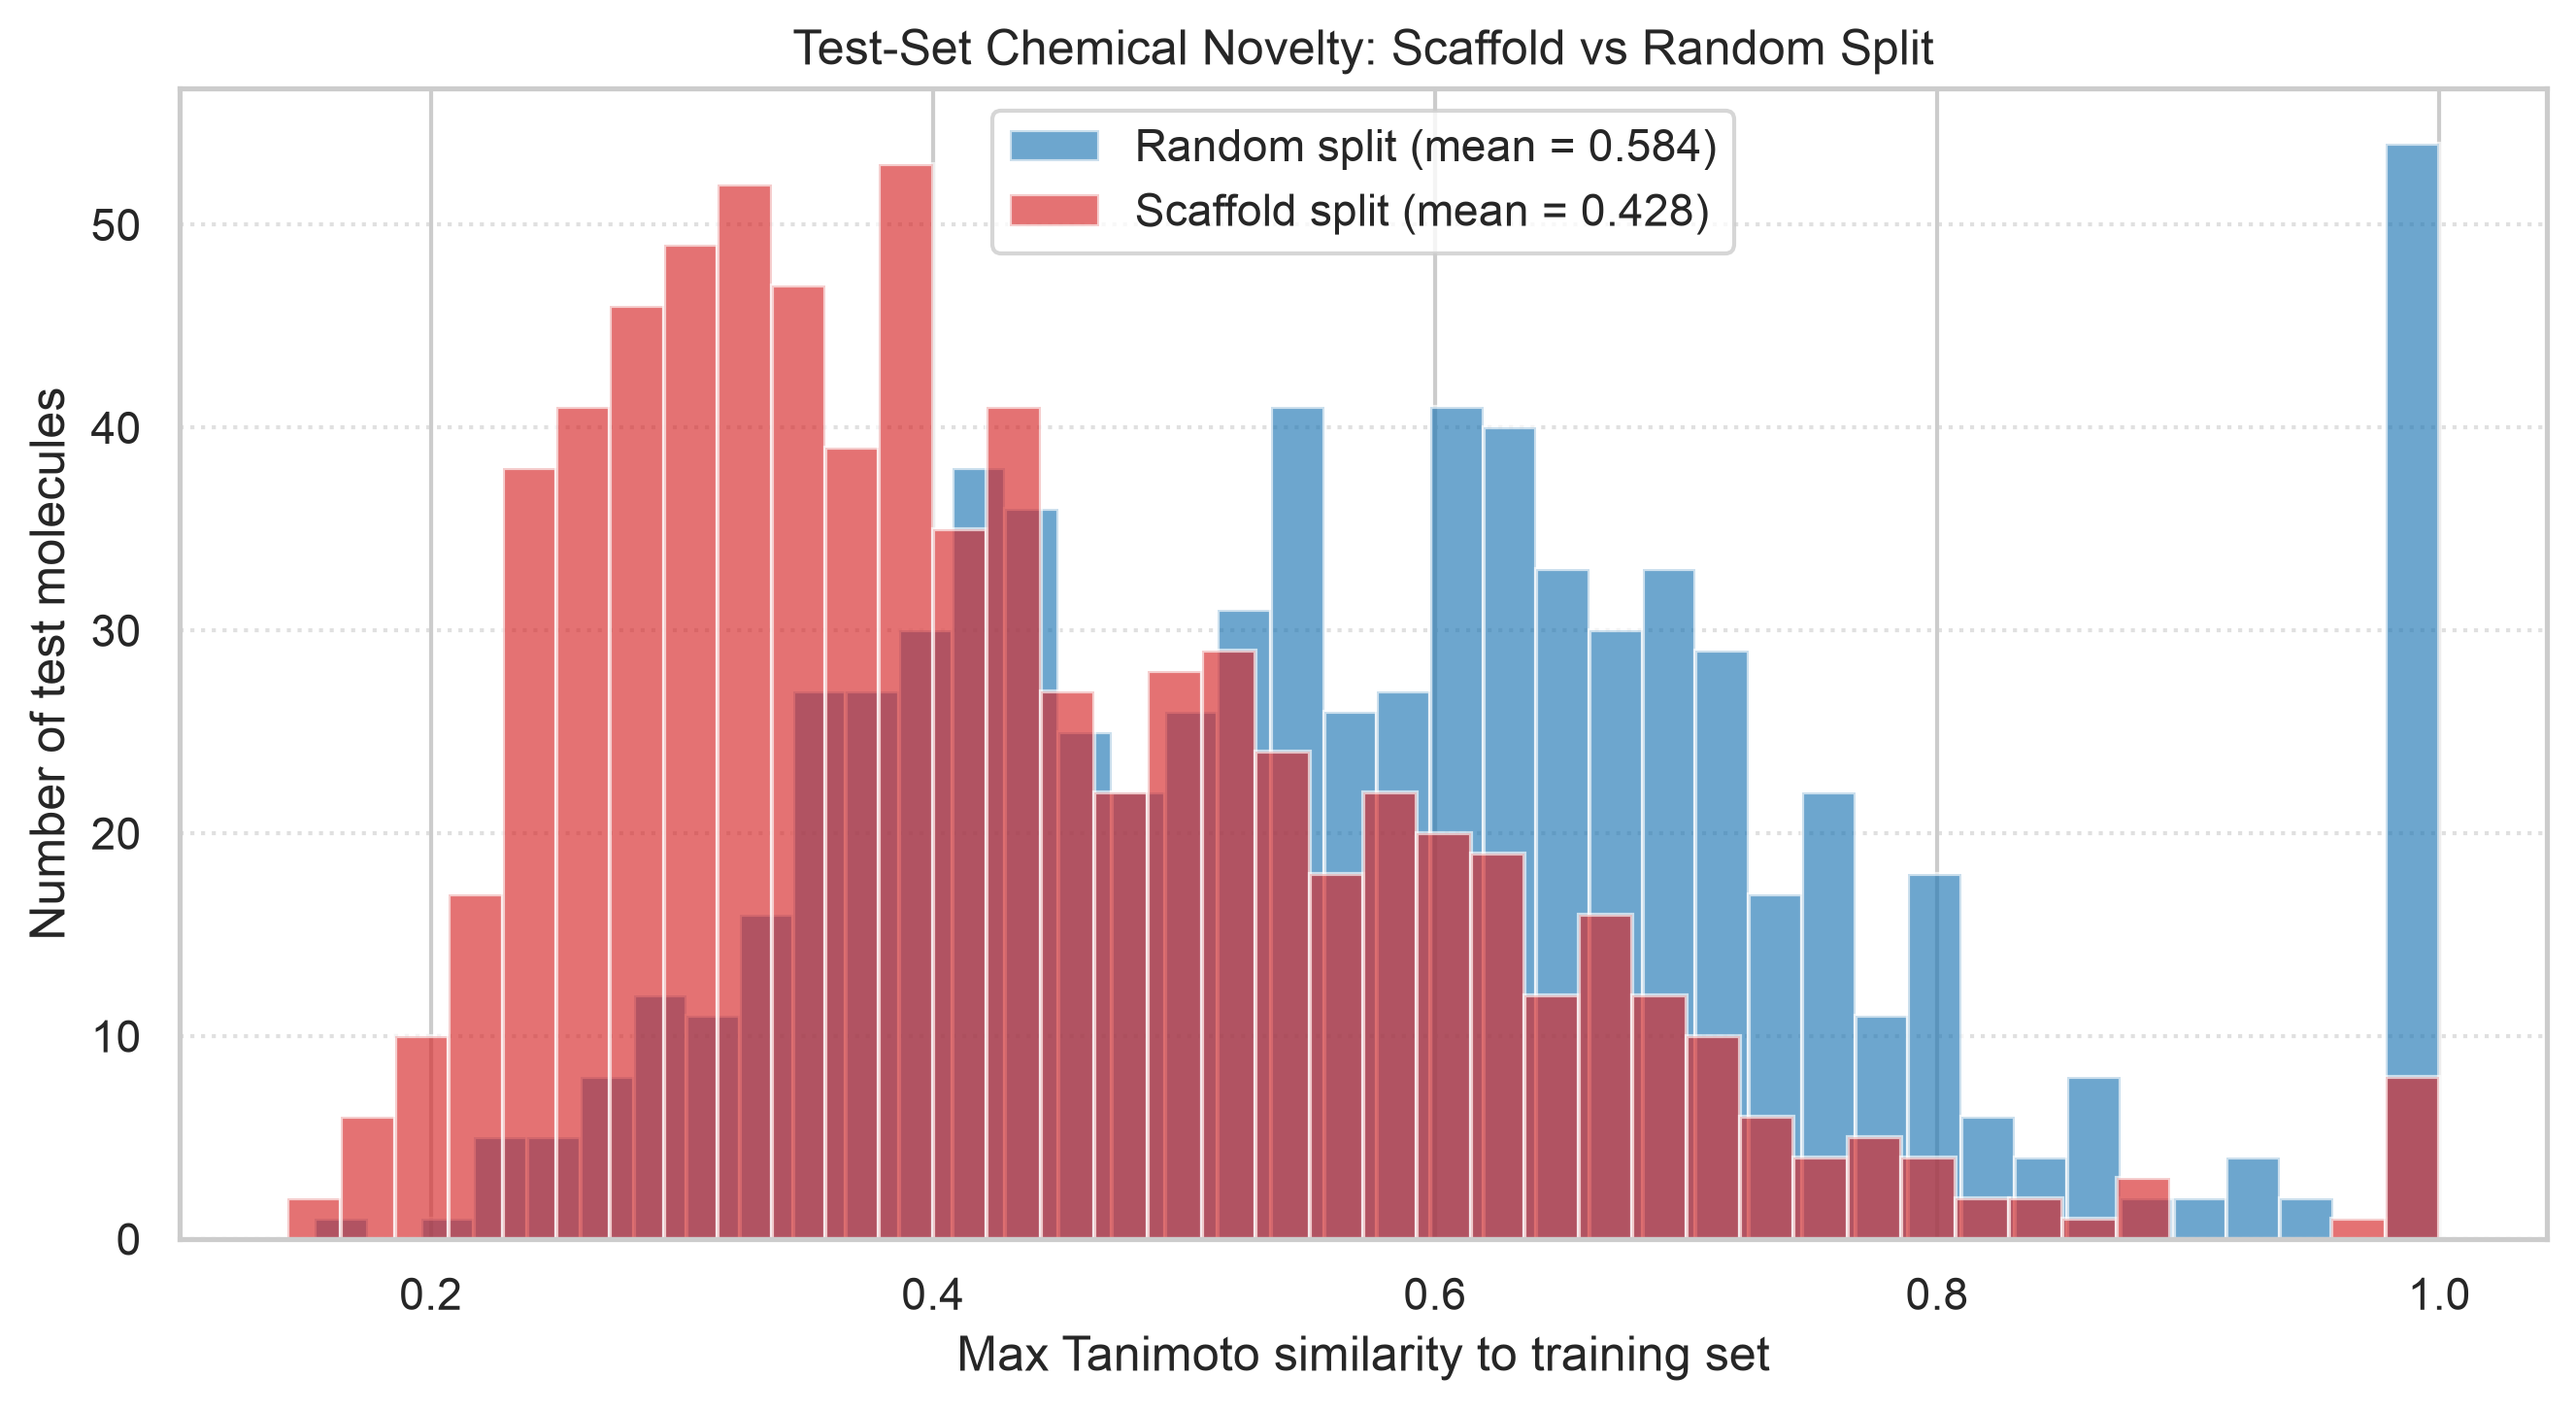
\includegraphics[width=0.95\columnwidth]{tanimoto_similarity_distributions.png}
\caption{Maximum Tanimoto similarity between test molecules and training molecules for the random and scaffold splits (2,048-bit Morgan fingerprints).}
\label{fig:tanimoto}
\end{figure}

\subsection{Generalization Gap: The Scaffold Split Penalty}
To evaluate the extent to which random splitting overestimates predictive generalization, we benchmarked the identical tuned configurations against the random split partition ($n=771$ test compounds). Table~\ref{tab:scaffold_penalty} and Figure~\ref{fig:scaffold_vs_random} contrast performance across both partitioning strategies.

\begin{table}[t]
\caption{Scaffold generalization penalty: Performance drop observed when transitioning from Random Split to Bemis--Murcko Scaffold Split (\texttt{morgan+desc}).}
\label{tab:scaffold_penalty}
\centering\small
\setlength{\tabcolsep}{3.5pt}
\begin{tabular}{@{}lrrrrrr@{}}
\toprule
Model & Scaf.\ ROC & Rand.\ ROC & $\Delta$ ROC & Scaf.\ PR & Rand.\ PR & $\Delta$ PR \\
\midrule
LogReg & 0.7317 & 0.8405 & -0.1088 & 0.3122 & 0.4818 & -0.1695 \\
Random Forest & 0.7762 & 0.8607 & \textbf{-0.0845} & 0.4035 & 0.5456 & \textbf{-0.1421} \\
XGBoost & 0.7606 & 0.8621 & -0.1015 & 0.4010 & 0.5647 & -0.1637 \\
\bottomrule
\end{tabular}
\end{table}

\begin{figure}[t]
\centering
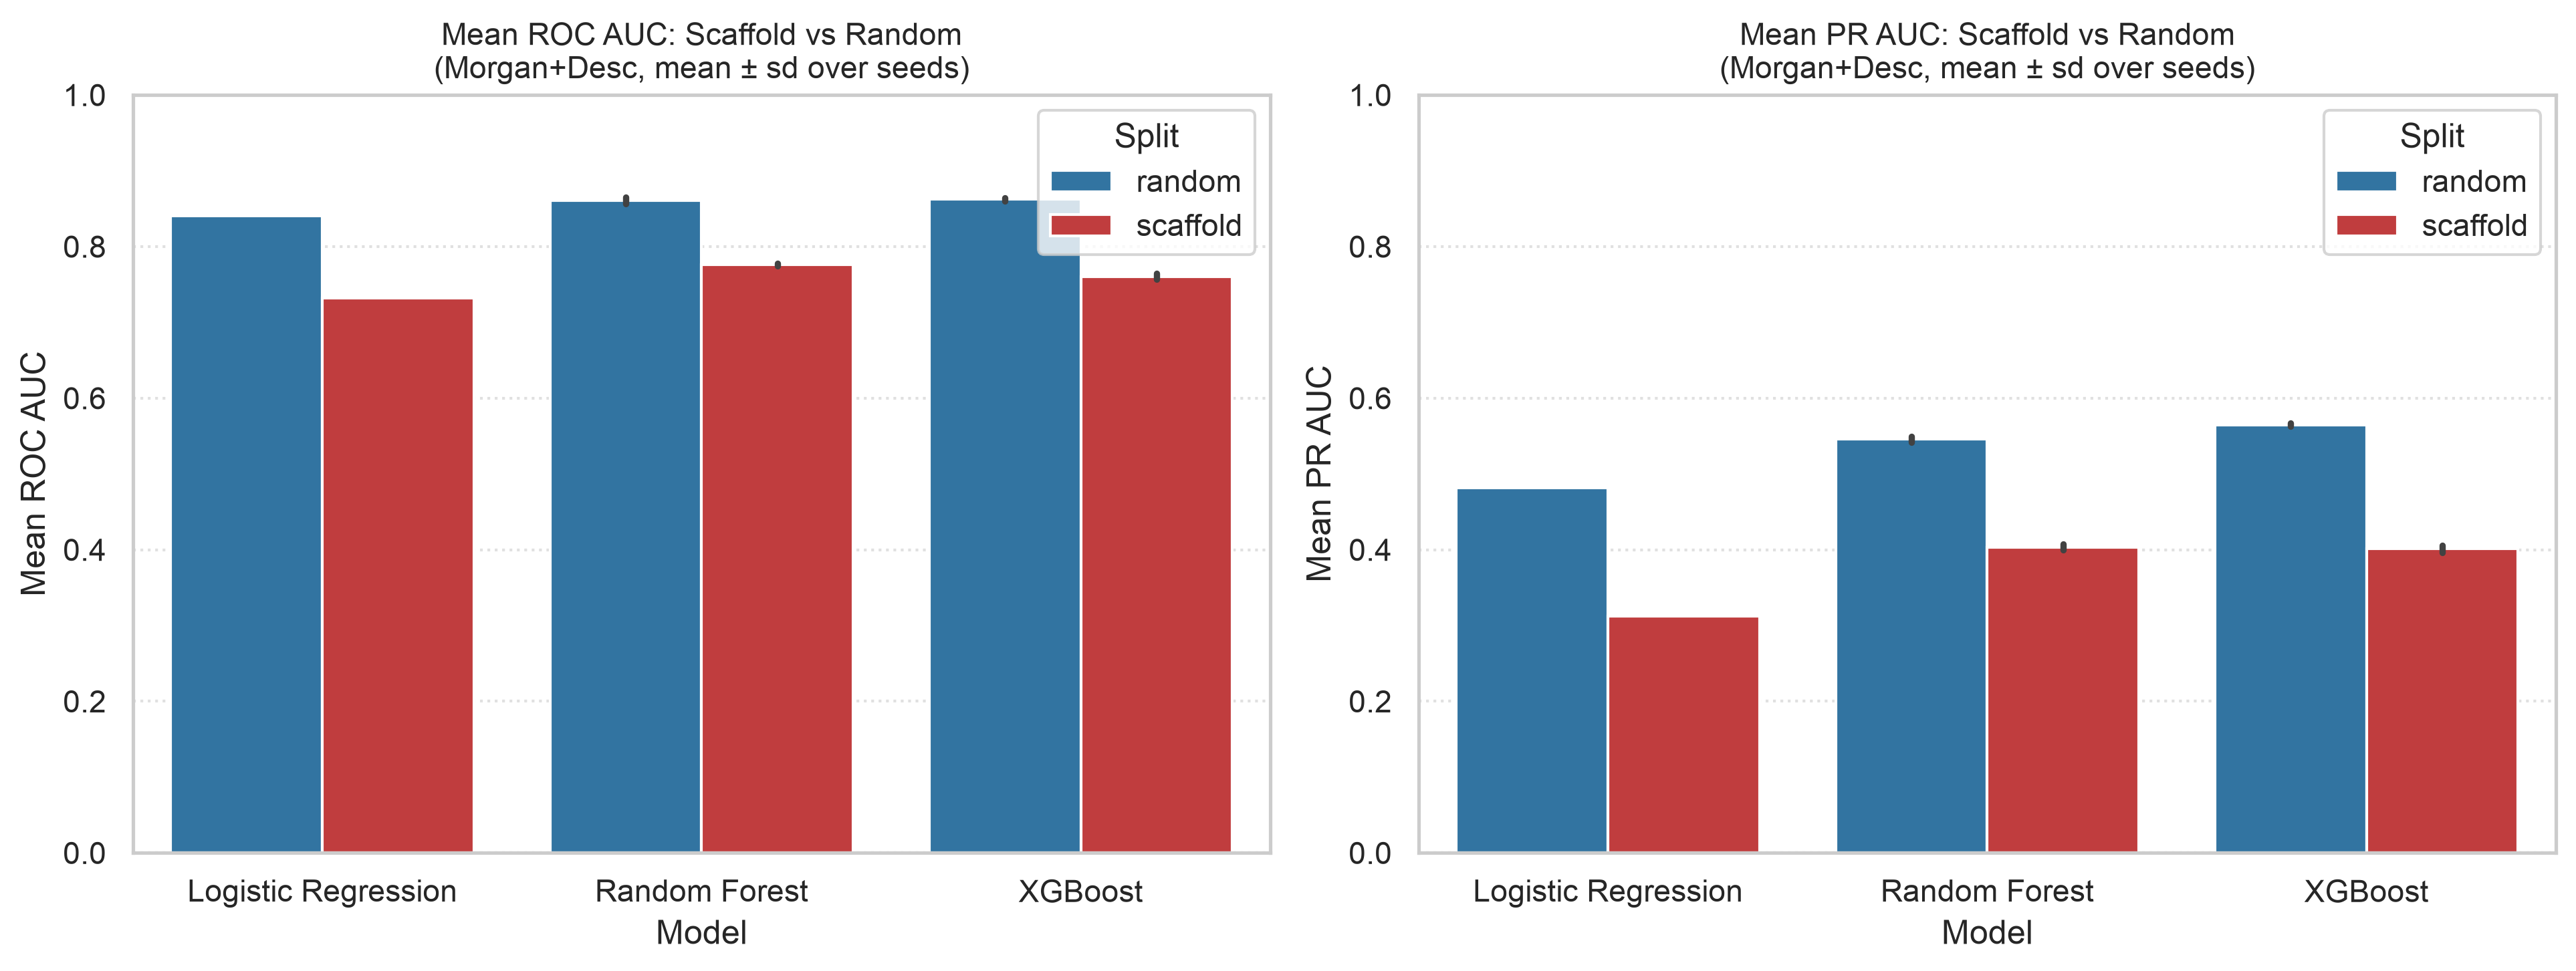
\includegraphics[width=0.98\columnwidth]{scaffold_vs_random_split.png}
\caption{Scaffold vs.\ Random split comparison across models on hybrid features (\texttt{morgan+desc}, mean $\pm$ sd over 3 seeds).}
\label{fig:scaffold_vs_random}
\end{figure}

All three architectures score lower on the scaffold split than on the random split (no significance test was run, and the two test sets contain different molecules):
\begin{itemize}
    \item On random splits, mean ROC AUCs are $0.84$--$0.86$ and mean PR AUCs are $0.48$--$0.56$ for the three models.
    \item When subjected to scaffold splitting, scores are lower: on hybrid features ROC AUC is $8.5$ to $10.9$ percentage points lower and PR AUC is $14.2$ to $17.0$ percentage points lower.
    \item On hybrid features Random Forest shows the smallest drop ($-0.0845$ in ROC and $-0.1421$ in PR); on Morgan-only features its ROC drop ($0.1076$) is the largest of the three models.
    \item This is consistent with the chemical novelty analysis in Section~\ref{subsec:novelty}, where scaffold test molecules are less similar to the training set. It is not a controlled test of leakage, because the two test sets contain different molecules and different numbers of positives.
\end{itemize}

\subsection{Per-Endpoint Performance and Biological Heterogeneity}
Toxicological predictability varies substantially across the 12 biological endpoints. Table~\ref{tab:endpoint_results_scaffold} and Figure~\ref{fig:endpoint_bars} detail individual test results on the scaffold split using hybrid features.

\begin{table*}[t]
\caption{Per-endpoint test performance on the scaffold split using hybrid representations (\texttt{morgan+desc}, mean $\pm$ sd over seeds 0, 1, 2; best ROC AUC per row in bold).}
\label{tab:endpoint_results_scaffold}
\centering\small
\setlength{\tabcolsep}{8pt}
\begin{tabular}{@{}llrrrr@{}}
\toprule
Endpoint Assay & Description & LR ROC AUC & RF ROC AUC & XGB ROC AUC & Top PR AUC (Model) \\
\midrule
NR-AR & Androgen receptor (full) & $0.691 \pm 0.000$ & $\mathbf{0.764 \pm 0.013}$ & $0.723 \pm 0.009$ & $0.464 \pm 0.009$ (XGB) \\
NR-AR-LBD & Androgen receptor (LBD) & $0.775 \pm 0.000$ & $0.838 \pm 0.016$ & $\mathbf{0.857 \pm 0.002}$ & $0.446 \pm 0.003$ (RF) \\
NR-AhR & Aryl hydrocarbon receptor & $0.806 \pm 0.000$ & $\mathbf{0.841 \pm 0.003}$ & $0.833 \pm 0.002$ & $0.596 \pm 0.002$ (RF) \\
NR-Aromatase & Cytochrome P450 19A1 & $0.695 \pm 0.000$ & $\mathbf{0.751 \pm 0.009}$ & $0.728 \pm 0.014$ & $0.367 \pm 0.005$ (RF) \\
NR-ER & Estrogen receptor alpha & $0.631 \pm 0.000$ & $\mathbf{0.685 \pm 0.004}$ & $0.674 \pm 0.011$ & $0.407 \pm 0.005$ (RF) \\
NR-ER-LBD & Estrogen receptor (LBD) & $0.705 \pm 0.000$ & $\mathbf{0.742 \pm 0.010}$ & $0.664 \pm 0.024$ & $0.310 \pm 0.006$ (RF) \\
NR-PPAR-gamma & Peroxisome proliferator & $0.708 \pm 0.000$ & $\mathbf{0.753 \pm 0.021}$ & $0.739 \pm 0.010$ & $0.339 \pm 0.012$ (RF) \\
SR-ARE & Antioxidant response & $0.702 \pm 0.000$ & $\mathbf{0.764 \pm 0.002}$ & $0.742 \pm 0.004$ & $0.526 \pm 0.013$ (RF) \\
SR-ATAD5 & Genotoxicity biomarker & $0.776 \pm 0.000$ & $\mathbf{0.777 \pm 0.017}$ & $0.757 \pm 0.010$ & $0.247 \pm 0.004$ (XGB) \\
SR-HSE & Heat shock response & $0.726 \pm 0.000$ & $\mathbf{0.739 \pm 0.003}$ & $0.727 \pm 0.012$ & $0.267 \pm 0.007$ (RF) \\
SR-MMP & Mitochondrial disruption & $0.836 \pm 0.000$ & $0.863 \pm 0.002$ & $\mathbf{0.879 \pm 0.004}$ & $0.640 \pm 0.004$ (XGB) \\
SR-p53 & p53 tumor suppressor & $0.730 \pm 0.000$ & $0.796 \pm 0.009$ & $\mathbf{0.806 \pm 0.007}$ & $0.361 \pm 0.001$ (XGB) \\
\bottomrule
\end{tabular}
\end{table*}

\begin{figure*}[t]
\centering
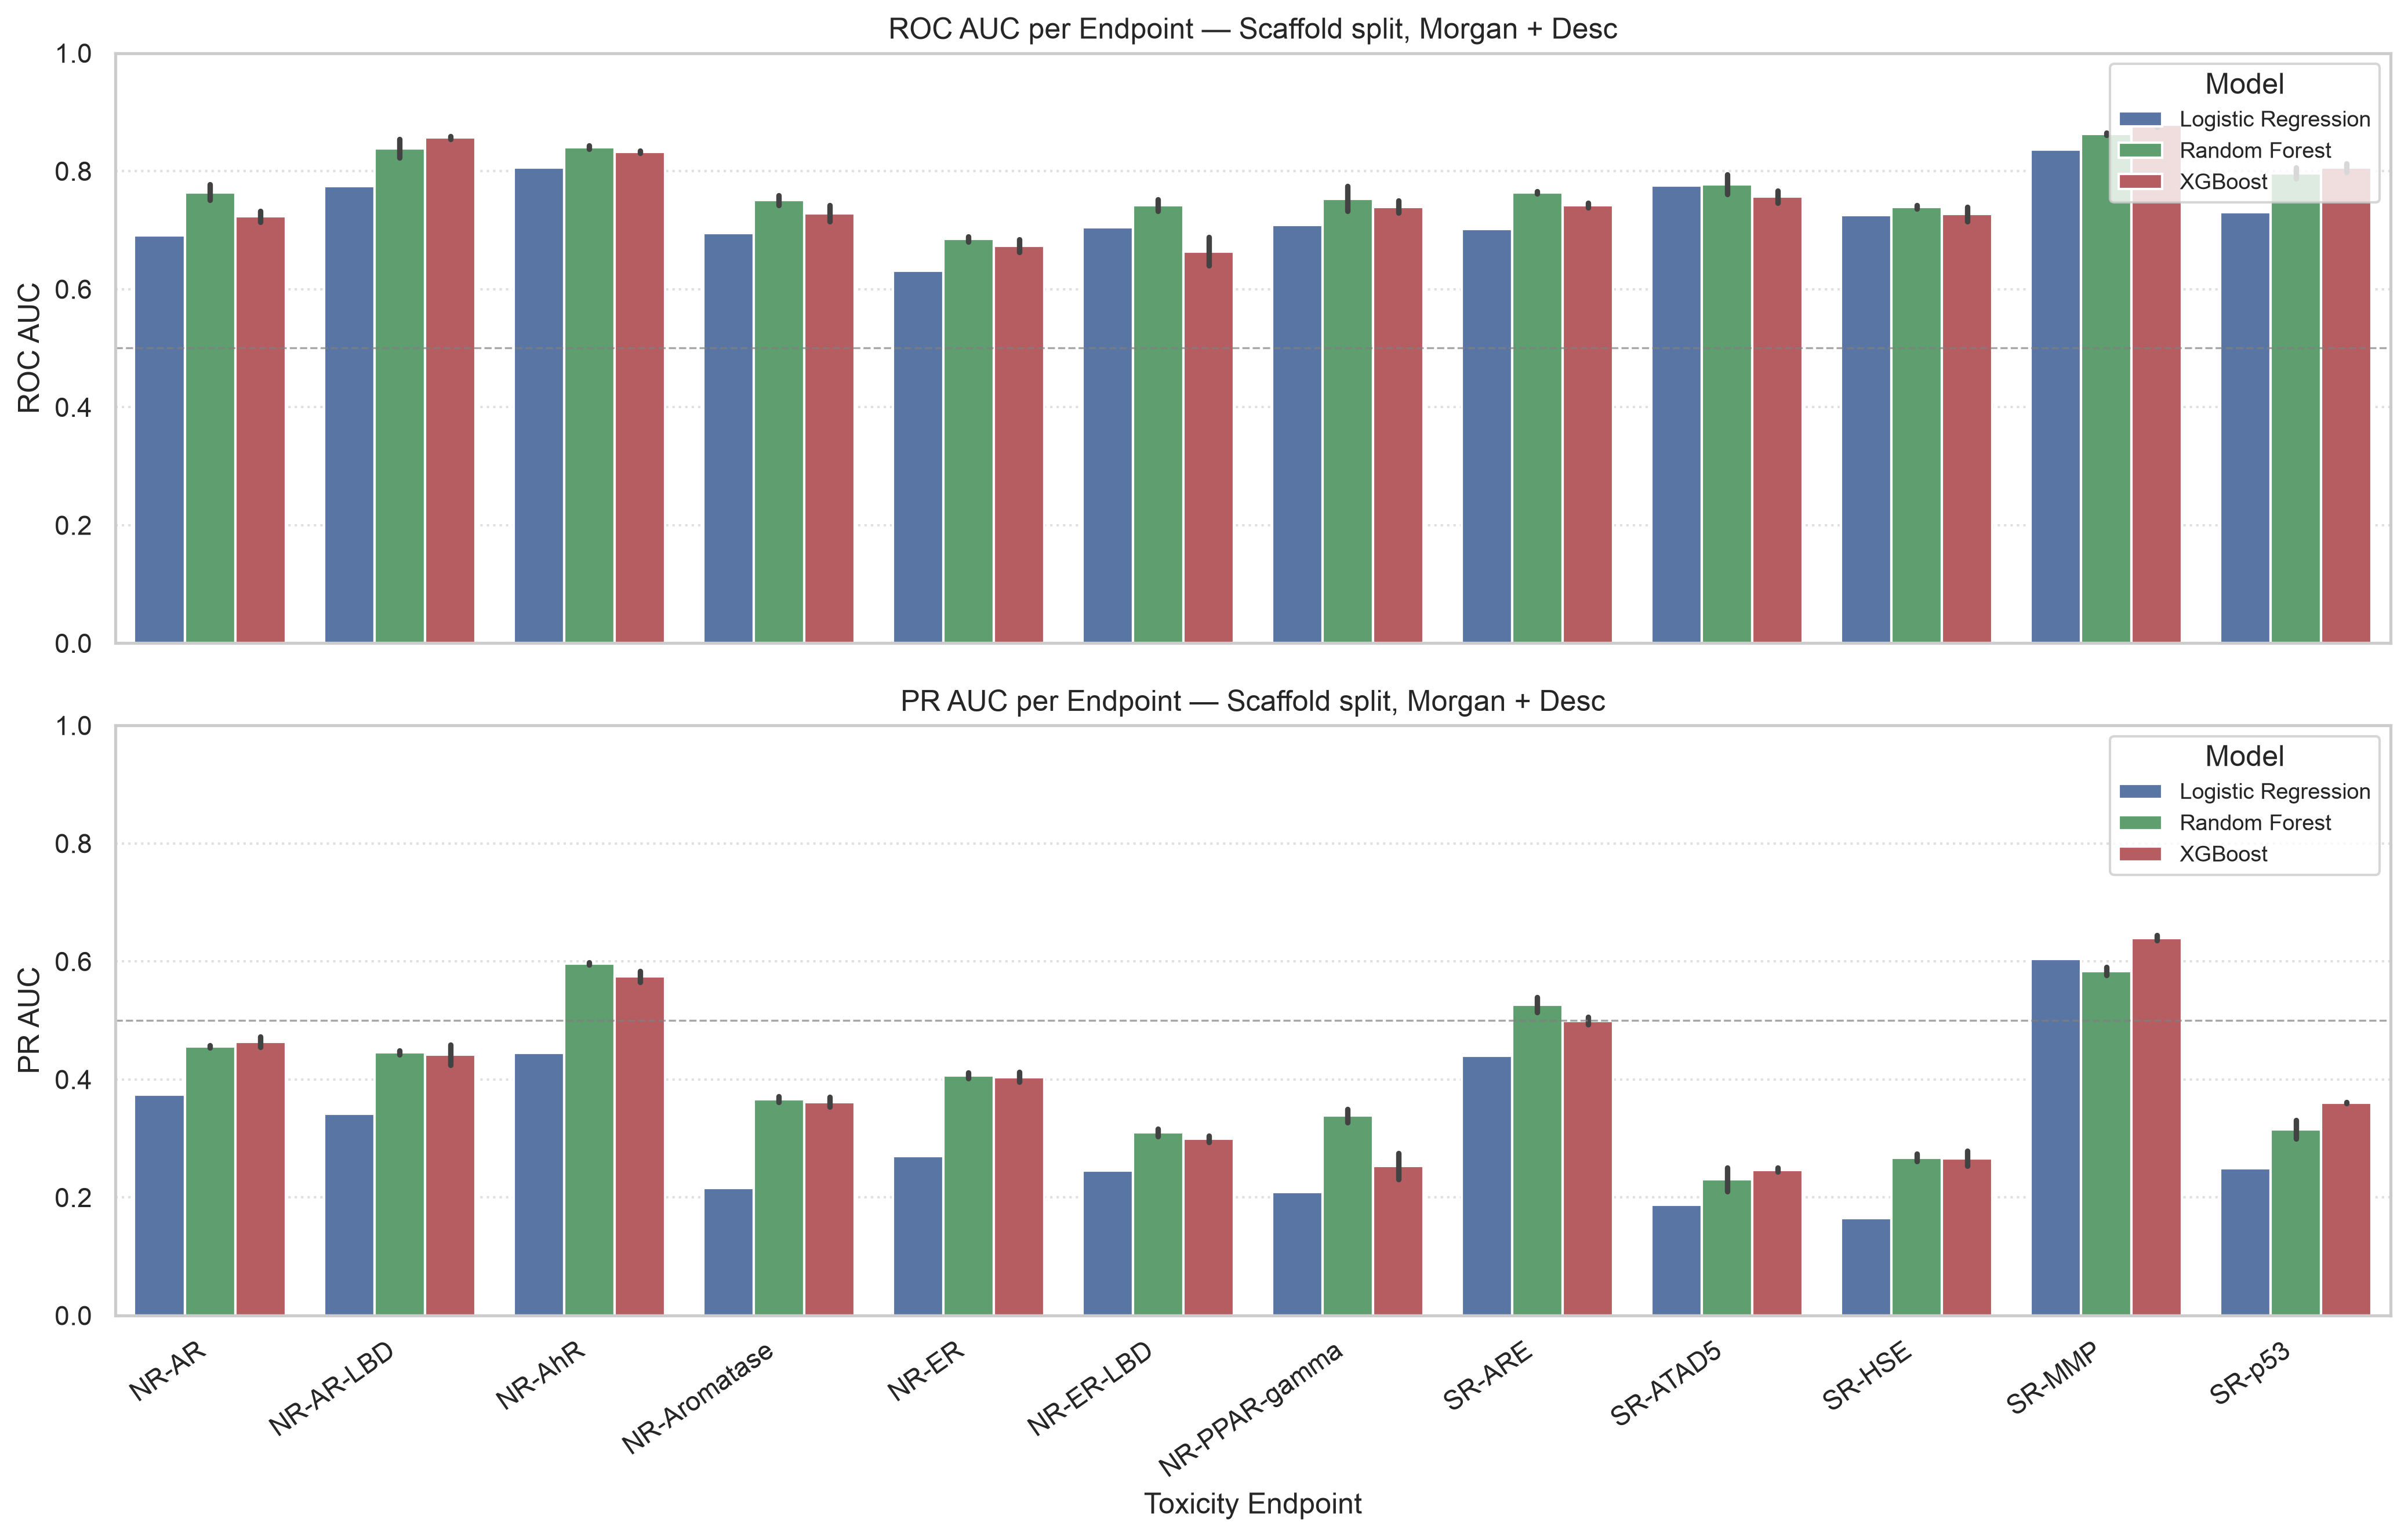
\includegraphics[width=0.98\textwidth]{endpoint_bars_scaffold_morgan_desc.png}
\caption{Per-endpoint test performance (ROC AUC top, PR AUC bottom) on the scaffold split using hybrid features (\texttt{morgan+desc}, mean $\pm$ sd over 3 seeds).}
\label{fig:endpoint_bars}
\end{figure*}

\subsubsection{High-Predictability Endpoints}
The bioassays exhibiting the strongest predictability are SR-MMP, NR-AhR, and NR-AR-LBD:
\begin{itemize}
    \item \textbf{SR-MMP (Mitochondrial Membrane Disruption):} Achieves top performance across the entire benchmark (XGBoost ROC AUC $0.8790 \pm 0.004$, PR AUC $0.6400 \pm 0.004$). We did not test why this endpoint is easier; one possibility is that lipophilicity-related descriptors such as $\log P$ and polar surface area carry signal for it.
    \item \textbf{NR-AhR (Aryl Hydrocarbon Receptor):} Random Forest achieves ROC AUC $0.8410 \pm 0.003$ and PR AUC $0.5960 \pm 0.002$. We did not test why this endpoint is predictable.
    \item \textbf{NR-AR-LBD:} XGBoost achieves ROC AUC $0.8570 \pm 0.002$, the highest ROC AUC among the nuclear-receptor endpoints; we did not investigate the cause.
\end{itemize}

\subsubsection{Challenging Endpoints}
Conversely, endpoints such as NR-ER, SR-HSE, and SR-ATAD5 proved substantially more challenging:
\begin{itemize}
    \item \textbf{NR-ER (Estrogen Receptor):} Has the lowest best-model ROC AUC across the 12 endpoints ($0.685 \pm 0.004$ with RF); we did not investigate why.
    \item \textbf{SR-HSE \& SR-ATAD5:} While exhibiting acceptable ROC AUCs ($\approx 0.74$--$0.78$), their PR AUCs remain low ($0.267$ and $0.247$, respectively). Active compounds are about $3.75\%$ of labeled SR-ATAD5 molecules and about $5.71\%$ of labeled SR-HSE molecules.
\end{itemize}
These endpoints are natural ones to watch when the Phase 2 graph models are compared against this baseline.

\section{Conclusion}
Phase 2 will investigate graph neural networks and hybrid molecular representations.


\bibliographystyle{IEEEtran}
\bibliography{references}

\end{document}
